\documentclass[conference]{IEEEtran}
% If the IEEEtran.cls has not been installed into the LaTeX system files,
% manually specify the path to it.  e.g.
% \documentclass[conference]{./IEEEtran}

% Add and required packages here
\usepackage{graphicx,times,amsmath}
\usepackage[utf8]{inputenc} 

% Correct bad hyphenation here
\hyphenation{op-tical net-works semi-conduc-tor IEEEtran}

% To create the author's affliation portion using \thanks
\IEEEoverridecommandlockouts

\textwidth 178mm
\textheight 239mm
\oddsidemargin -7mm
\evensidemargin -7mm
\topmargin -6mm
\columnsep 5mm

\begin{document}

% Project title: keep the \ \\ \LARGE\bf in it to leave enough margin.
\title{\ \\ \LARGE\bf Development of AI Ms. Pac-Man Controllers}

\author{Julian Møller}

% Uncomment out the following line for invited papers
%\specialpapernotice{(Invited Paper)}

% Make the title area
\maketitle

\begin{abstract}
In this paper, successful implementations of two Ms. Pac-Man controllers and unsuccessful implementation of one Ms. Pac-Man controller is described. The methodologies used are genetic evolution of state machines, Monte Carlo Tree Search and Multilayered Perceptron.
The results of the implementations will be described as well as their shortcomings. Comparisons will be made with the benchmark controllers
\emph{StarterGhosts}, \emph{Legacy} and \emph{Legacy2TheReckoning}. Maximum scores of approximately 14.000 (with means around 6.500 points)
are obtained against the toughest ghosts.
\end{abstract}

\section{Introduction}
In this paper I will describe the controllers I have developed for the real-time arcade game Ms. Pac-Man (henceforth named Pac-Man).

I will first describe the state based controller which was evolved via genetic programming. Then, I will describe the Monte Carlo Tree
Search controller and lastly, I will describe my failed attempts at making a controller based on a multilayered perceptron network. In
the end, I will discuss the project and evaluate my results.

\section{Genetically Evolved State Machine}

The basis of the genetically evolved state machine controller (the SMC) is the division of labour into the following distinct states:
\begin{itemize}
\item Go to pill
\item Go to powerpill
\item Hunt ghosts
\item Go to safest node
\end{itemize}

All states have a method which is used to determine if the state can handle the current game state. The states also have a built in
priority which changes the order in which the states are checked for validity. The states uses a number of evolvable parameters. These
are used when determining if the states can handle the game state and when a appropriate move is calculated. The
priorities for the states are also evolvable.

The parameters used for the different states are:

\begin{itemize}
\item \textbf{Go to pill}: Priority, distance to nearest ghost, distance to nearest pill
\item \textbf{Go to power pill}: Priority, minimum distance to nearest ghost,  maximum distance to nearest ghost, distance to nearest power pill
\item \textbf{Hunt ghosts}: Priority, minimum remaining edible time, distance to nearest edible ghost
\item \textbf{Go to safest node}: Priority
\end{itemize}

\subsection*{Evolution}

The evolution of the parameters was performed by creating a population of 100 genomes. Each iteration these were evaluated. Of these, the
50 worst were eliminated. They were replaced with 20 entirely new genomes, 20 mutations of the best 20 genomes and 10 crossovers based on
pairs from the 20 best genomes. 100 evolutions were run. The average score assigned to a genome was calculated based on the average of the
previous iterations and the average of the newest iteration.

\subsection*{Problems and ways to improve}

The controller was evolved against single opponents. This led to overfitting of the problem, witnessed by the fact that none of the evolved
controllers were consistently good against all other controllers.

The search space for the genome was on top of that too large. Every part of the genome started in the range 0-200. For some of the
parts of the genome this might not have been a sufficiently large range, whereas for others the range was too big. The result of this is
that ranges of values for the genome parts might have been superfluous.

\section{Monte Carlo Tree Search}

Monte Carlo Tree Search is a 'best first' way to get an estimate of the results of actions in a search space, where the space is too large to construct a full tree of actions and outcomes.

It works by recursively selecting actions and playing out their outcomes based on random actions.
One of the advantages of Monte Carlo Tree Search is that the algorithm can be terminated at any time, because the current best choice will always be known. Given infinite time, the outcome simulation will converge towards an optimal solution.

My implementation utilizes the default policies (\emph{TreePolicy} and \emph{DefaultPolicy}) for expansion and playout. The implementation
constructs nodes at each possible move for Pac-Man. The \emph{DefaultPolicy} is modified a bit from completely random playout. Pac-Man is only allowed to go straight ahead when in corridors, except when a ghost has just been eaten or when a ghost is very near by. Otherwise, all direction changes take place at junctions. Pac-Man isn't allowed to go backwards at junctions either, to avoid the search space becoming larger than it already is.

\subsection*{Problems and ways to improve}

Because the nodes in the search tree is based on individual moves, Pac-Mans strategy becomes a micro-strategy and doesn't allow for Pac-Man to look ahead in the future. The first an best way to improve the implementation is to change the tree from being based on moves to being based on junctions like described in \cite{enhancements}. Another good way to improve the implementation is to change the selection of
child nodes to use a heurestic function instead of relying on randomness.

\section{Multilayered Perceptron Network}

My implementation of this controller failed, so the following is what I would have done, had I gotten the neural network to function. The neural network implementation is included in the archive with source code. I tried to follow the algorithm from \cite{aima}, page 734, but something unfortunately went wrong.

Multilayered perceptron networks is a machine learning technique, where a number of inputs are passed through a network and results in a number of outputs, representing what the network has been taught.

This can for instance be utilized in Pac-Man to determine a 'goodness' score for a given state, and by feeding the neural network each possible move as a distinct state, determine which is the better action to perform. A neural network can also be used to determine which state it is favorable for Pac-Man to be in (such as flee, eat pill, seek power pill or hunt ghost). The underlying control structure can then be a simple state machine where the active state is determined by the neural network. I would have chosen the former solution, as it is simpler to train the neural network either by manually playing games or by letting another AI controller play. If the latter solution is to be utilized, it requires an AI controller, that at each state is able to properly determine which state it is favorable to be in.

\subsection*{Planned implementation}

I would have started evaluation of the MLP network with the following inputs (to match my state machine controller):

\begin{itemize}
\item Distance to nearest regular ghost
\item Distance to nearest edible ghost
\item Distance to nearest pill
\item Distance to nearest power pill
\end{itemize}

Other input values that could be explored are:

\begin{itemize}
\item Is Pac-Man at a junction?
\item Current score
\item Number of ghosts eaten
\item Is (the nearest) ghost ahead of or behind Pac-Man
\item Where in the maze is Pac-Man?
\end{itemize}

\subsection*{Primary problems}

A problem with a MLP network is determining the topology of the network, as there is no known way to determine beforehand if a topology will be a good fit for a certain problem space. This could be 'solved' by utilizing genetic programming and letting an algorithm evolve the topology based on the achieved scores in the game.

Another problem is that MLP networks suffer from overfitting, which requires multiple distinct sets of data for training, test and verification. To get consistent results, this requires a consistent controller used for training.

\section{Results}

\subsection{Evolution of genomes for the SMC}

Figures \ref{fig-evos}, \ref{fig-evol} and \ref{fig-evol2} show the average score of the controller as the evolution progressed. The controller reached a quite stable score against all three ghosts. The StarterGhosts were more forgiving with regards to genome parameters than the Legacy and Legacy2 ghosts, as the average score was quite high to begin with. For all three simulations, a 'maximum' fitness was reached quite early.

\begin{figure}[htp]
\centerline{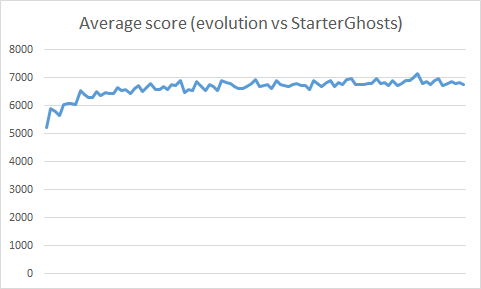
\includegraphics[width=0.9\columnwidth]{s_evo.png}}
\caption{Evolution vs. StarterGhosts}
\label{fig-evos}
\end{figure}

\begin{figure}[htp]
\centerline{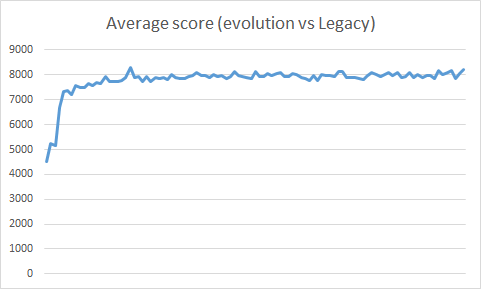
\includegraphics[width=0.9\columnwidth]{l_evo.png}}
\caption{Evolution vs. Legacy}
\label{fig-evol}
\end{figure}

\begin{figure}[htp]
\centerline{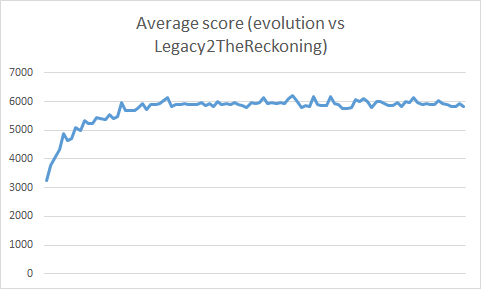
\includegraphics[width=0.9\columnwidth]{l2_evo.png}}
\caption{Evolution vs. Legacy2TheReckoning}
\label{fig-evol2}
\end{figure}

\subsection{Performance against ghosts}

Figure \ref{fig-avgs} shows the performance against the starter ghosts. \emph{S}, \emph{L} and \emph{L2} represent that the values for the genome are the ones found to be best against StarterGhosts, Legacy and Legacy2TheReckoning, respectively.

The most stable performer is the MCTS controller, but due to its micro- instead of macro-strategy, it doesn't score very high. All three genomes for the state machine performs better than StarterPacMan, but both StarterPacMan and all three state machines have a quite large standard deviance. The L2 version performs about as well as the version evolved against the ghosts specifically, but has a higher standard deviation.

Figure \ref{fig-avgl} show the same pattern: The controllers perform about the same, with an advantage for the SMC that was specifically evolved to handle the Legacy ghosts.

Another picture is painted in figure \ref{fig-avgl2}, where the SMC specifically evolved show a much higher average score than the rest of the controllers. I believe this can both be because the ghosts have a very distinct behavior, but also because the ghosts are less forgiving, so a specialized version will perform better.

Figure \ref{fig-cvals} show the average scores for the MCTS controller based on different values for the C-component, that determine the rate of exploration vs exploitation when the search tree is traversed. The most solid value is $C = 0.2$, which displays the lowest variance of all of my controllers, but an optimal C-value requires more extensive testing than I have performed.\footnote{Because the MCTS utilized all available time given, the games were very slow, so it wasn't feasible to run that many simulations.}

\begin{figure}[htp]
\centerline{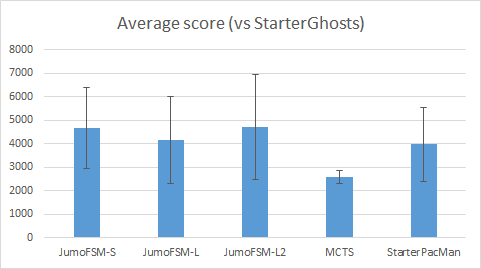
\includegraphics[width=0.9\columnwidth]{average_starter.png}}
\caption{Average score against StarterGhosts}
\label{fig-avgs}
\end{figure}

\begin{figure}[htp]
\centerline{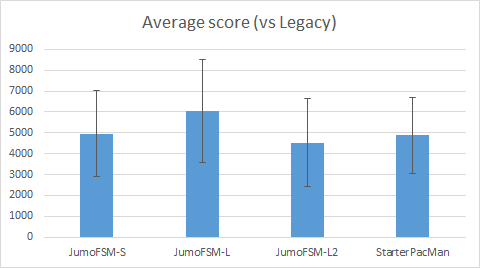
\includegraphics[width=0.9\columnwidth]{average_legacy.png}}
\caption{Average score against Legacy}
\label{fig-avgl}
\end{figure}

\begin{figure}[htp]
\centerline{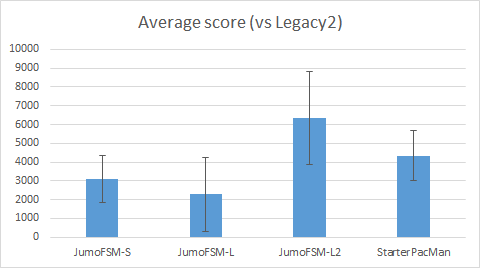
\includegraphics[width=0.9\columnwidth]{average_legacy2.png}}
\caption{Average score against Legacy2TheReckoning}
\label{fig-avgl2}
\end{figure}

\begin{figure}[htp]
\centerline{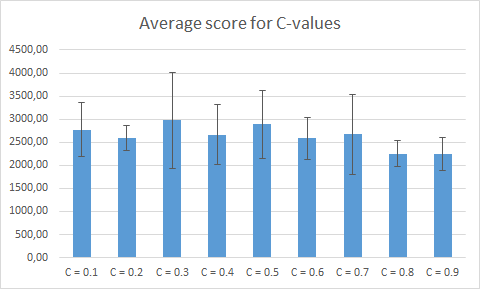
\includegraphics[width=0.9\columnwidth]{c_values.png}}
\caption{Average score against StarterGhosts for different C-values}
\label{fig-cvals}
\end{figure}

\section{Conclusions}

I set out to create a SMC that performed better than the starter ghosts, which I did, so I am happy about that.
I would have liked to create a macro-based MCTS controller instead of the micro-based one I implemented, to score better, but I am happy with the high stability and low standard deviance the controller exhibited.

I am not satisfied, that I couldn't get the MLP network to work, as that is the solution I think is the most interesting. I underestimated how long time it could take to debug the MLP implementation. I also wasted too much time on improving the state based controller, that I should have used on the MLP and on making the MCTS better.

% Trigger a \newpage just before a given reference number in order to
% balance the columns on the last page.  Adjust the value as needed;
% it may need to be readjusted if the document is modified later.
%\IEEEtriggeratref{8}
% The "triggered" command can be changed if desired:
%\IEEEtriggercmd{\enlargethispage{-5in}}

% The references section can either be generated by hand or by an
% automatic tool like BibTeX.  If using BibTex, use the standard IEEEtran
% bibliography style.
%\bibliographystyle{IEEEtran.bst}
%
% The argument to \bibliography is/are the name(s) of your BibTeX file(s)
% that contains string definitions and bibliography database(s).
%\bibliography{IEEEabrv,SamplePaper}
%
% If you generate the bibliography by hand, or if you copy in the
% resultant .bbl file, set the second argument of \begin to the number of
% references in the bibliography (used to reserve space for the reference
% number labels box).

\begin{thebibliography}{3}
\bibitem{aima}
S.~Russel, P.~Norvig \emph{Artificial Intelligence - A Modern Approach}.\hskip 1em plus 0.5em minus 0.4em\relax
  Pearson, 2010.

\bibitem{enhancements}
T.~Pepels, M.H.M.~Winands, ``Enhancements for Monte-Carlo Tree Search in Ms Pac-Man,''
\end{thebibliography}

% That's all folks...
\end{document}
